% Drawing 154/05-4 -- folder 154, batch 05, archive page 94 (PDF page 95).
% Transcription: en haut à gauche, au crayon, un croquis : des droites concourantes en un point, trois petits triangles marqués $\sigma_0$, $\sigma_1$, $\sigma_2$ ; au-dessous, une accolade (un arc) sur la suite « $\sigma_0\ \sigma_f\ \sigma_1\ \sigma_s\ \sigma_2$ », chaque terme surmonté d'un point, les indices $f$ et $s$ surchargés et un sixième terme raturé. Au centre, deux dessins en couleur de la même carte (arêtes vert clair et bleues) : un sommet où se rencontrent des arêtes des deux couleurs, un triangle colorié en orange et les secteurs voisins marqués $\sigma_0$, $\sigma_1$, $\sigma_2$, $\sigma_f$, $\sigma_s$, hachurés en gris dans le second. À droite, une ligne brisée vert clair marquée de petits traits rouges et de deux points d'exclamation, un pentagone au crayon, et, en bas, un faisceau de droites grises aboutissant à une courbe vert clair marquée de traits rouges, étiquetée « $\sigma_s$ »
% Kind: pencil sketch of sectors; two drawings of a two-coloured map; broken line and pencil fan. Method 2 (schematic redraw from the facsimile). Status: partial.
% Notes: Top left, in pencil: lines concurrent at a point, small triangles marked sigma_0, sigma_1, sigma_2, and below an arc over the sequence « sigma_0 sigma_f sigma_1 sigma_s sigma_2 » (each term with a dot above; the overwritten indices and the struck sixth term are not reproduced). Centre: two drawings of the same map, edges light green and blue: a vertex where edges of both colours meet, a triangle coloured orange and the neighbouring sectors marked sigma_0, sigma_1, sigma_2, sigma_f, sigma_s (hatched grey in the second, left out). Right: a light green broken line with small red strokes and two exclamation marks, a pencil pentagon, the pencilled legend with sigma_s, sigma_alpha, sigma_r (given as text), and at the bottom a pencil fan of grey lines ending on a light green curve with red strokes, labelled sigma_s. Read from the page view; the two maps are schematic (the edges are placed approximately). Still differs from the facsimile: Top left, in pencil: lines concurrent at a point, small triangles marked sigma_0, sigma_1, sigma_2, and below an arc over the sequence « sigma_0 sigma_f sigma_1 sigma_s sigma_2 » (each term with a dot above; the overwritten indices and the struck sixth term are not reproduced). Centre: two drawings of the same map, edges light green and blue: a vertex where edges of both colours meet, a triangle coloured orange and the neighbouring sectors marked sigma_0, sigma_1, sigma_2, sigma_f, sigma_s (hatched grey in the second, left out). Read from the page view; the two maps are schematic (the edges are placed approximately). 3 coloured or hatched triangle(s) are placed schematically and are not bounded by the strands that bound them on the page.
% Coordinates: 1 unit = 1 mm = 1/100 of the crop width (bbox in page fractions: [0.175, 0.079, 0.964, 0.438]).
% Redrawn by Claude (claude-opus-5-5), issue #73, 2026-11-07; not checked by a human; not compiled (no TeX in the session).
% Revised by Claude (claude-opus-5-5) 2026-11-09 (issue #128) after Michel's check: vertices snapped to exact intersections (drawn points on their lines, meeting ends on the stroke they meet, near-concurrent lines through one computed point, curve ends on their rim); labels at \small as in folder 80 batch 3. Status: partial.
% Rights: reproduces part of the work -- behind RENDER_TRANSCRIPTS, never published by itself.
\documentclass[tikz,border=3pt]{standalone}
\usepackage{amsmath,amssymb}
\usetikzlibrary{patterns,arrows.meta}
\tikzset{Or/.style={orange!90!black}, Ye/.style={yellow!80!orange}, Lg/.style={green!60!black!70}, Dg/.style={green!45!black}, Br/.style={brown!80!black}, Rd/.style={red!85!black}, Bl/.style={blue!70!black}, Gy/.style={black!40}, pencil/.style={black!45}, struck/.style={black!35}, mark/.style={circle,draw,inner sep=1.3pt}, pt/.style={circle,fill,inner sep=0.9pt}, opt/.style={circle,draw,fill=white,inner sep=1.1pt}}
\begin{document}
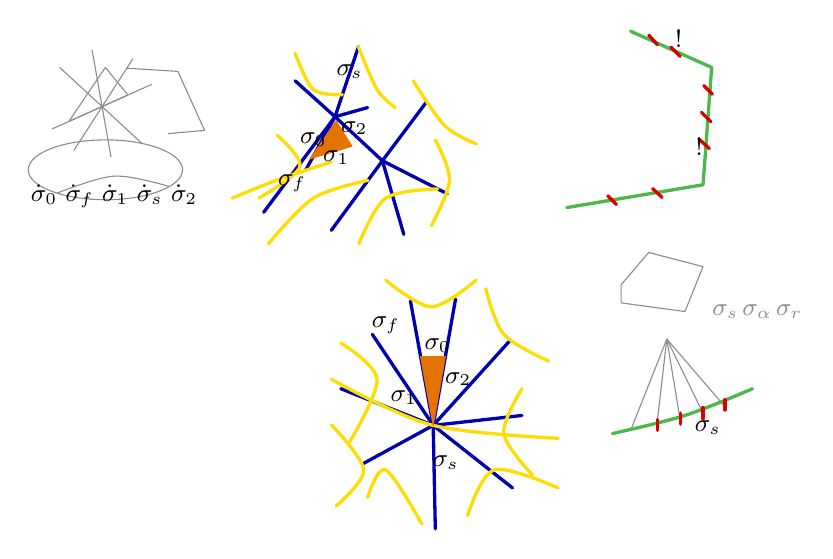
\begin{tikzpicture}[x=1mm,y=1mm,line cap=round,line join=round,font=\scriptsize]
\draw[pencil] (4.76,-13) -- (17.38,-7.35);
\draw[pencil] (7.52,-15.71) -- (14.97,-4.13);
\draw[pencil] (12.21,-16.58) -- (9.81,-2.98);
\draw[pencil] (16.15,-14.86) -- (5.7,-5.2);
\draw[pencil] (6.85,-12.07) -- (11.5,-5.2) -- (14.36,-8.7) -- cycle;
\draw[pencil] (11.5,-18.2) ellipse[x radius=9.8, y radius=3.8];
\node[inner sep=1pt] at (12.6,-21.6) {\small $\dot\sigma_0\ \dot\sigma_f\ \dot\sigma_1\ \dot\sigma_s\ \dot\sigma_2$};
\draw[pencil] plot[smooth, tension=0.55] coordinates {(5.37,-21.16) (12.6,-19) (19.63,-20.32)};
\draw[pencil] (14.21,-5.3) -- (20.7,-5.7) -- (24.1,-13.2) -- (19.5,-13.6);
\draw[Bl,very thick] (40.66,-11.46) -- (35.6,-6.9);
\draw[Bl,very thick] (40.66,-11.46) -- (43.64,-2.58);
\draw[Bl,very thick] (40.66,-11.46) -- (44.8,-10.3);
\draw[Bl,very thick] (40.66,-11.46) -- (46.68,-17.05);
\draw[Bl,very thick] (40.66,-11.46) -- (36.94,-18.24);
\draw[Bl,very thick] (40.66,-11.46) -- (31.6,-23.6);
\draw[Bl,very thick] (46.68,-17.05) -- (54.91,-21.24);
\draw[Bl,very thick] (46.68,-17.05) -- (49.4,-26.4);
\draw[Bl,very thick] (46.68,-17.05) -- (40.19,-25.89);
\draw[Bl,very thick] (46.68,-17.05) -- (52.24,-9.64);
\draw[Ye,very thick] plot[smooth, tension=0.55] coordinates {(35.6,-3.4) (37.9,-8) (41.6,-8.66)};
\draw[Ye,very thick] plot[smooth, tension=0.55] coordinates {(43.64,-2.58) (46,-8) (48.3,-10.3)};
\draw[Ye,very thick] plot[smooth, tension=0.55] coordinates {(50.6,-6.9) (54.6,-12.6) (58.6,-14.9)};
\draw[Ye,very thick] plot[smooth, tension=0.55] coordinates {(27.6,-21.8) (33.3,-19.5) (40.2,-17.2)};
\draw[Ye,very thick] plot[smooth, tension=0.55] coordinates {(32.2,-27.6) (37.9,-21.8) (44.85,-19.54)};
\draw[Ye,very thick] plot[smooth, tension=0.55] coordinates {(43.7,-27.6) (47.1,-21.8) (53.71,-20.63)};
\draw[Ye,very thick] plot[smooth, tension=0.55] coordinates {(53.4,-14.4) (55.2,-19.5) (52.9,-25.3)};
\draw[Ye,very thick] plot[smooth, tension=0.55] coordinates {(33.3,-13.8) (36.2,-17.8) (31,-21.8)};
\draw[Or] (37.5,-16.8) -- (40.8,-12) -- (42.8,-15.2) -- cycle;
\fill[pattern=north east lines,Or] (37.5,-16.8) -- (40.8,-12) -- (42.8,-15.2) -- cycle;
\node[inner sep=1pt] at (37.9,-14.4) {\small $\sigma_0$};
\node[inner sep=1pt] at (43.1,-12.9) {\small $\sigma_2$};
\node[inner sep=1pt] at (40.8,-16.7) {\small $\sigma_1$};
\node[inner sep=1pt] at (35.2,-19.9) {\small $\sigma_f$};
\node[inner sep=1pt] at (42.5,-5.7) {\small $\sigma_s$};
\draw[Bl,very thick] (53.13,-50.66) -- (50.24,-34.85);
\draw[Bl,very thick] (53.13,-50.66) -- (55.97,-34.61);
\draw[Bl,very thick] (53.13,-50.66) -- (62.89,-39.88);
\draw[Bl,very thick] (53.13,-50.66) -- (64.4,-49.4);
\draw[Bl,very thick] (53.13,-50.66) -- (63.2,-58.6);
\draw[Bl,very thick] (53.13,-50.66) -- (53.4,-63.8);
\draw[Bl,very thick] (53.13,-50.66) -- (44.17,-55.55);
\draw[Bl,very thick] (53.13,-50.66) -- (41.4,-46);
\draw[Bl,very thick] (53.13,-50.66) -- (45.4,-39.1);
\draw[Ye,very thick] plot[smooth, tension=0.55] coordinates {(41.4,-40.2) (46,-44.8) (42.52,-52.76)};
\draw[Ye,very thick] plot[smooth, tension=0.55] coordinates {(47.1,-32.2) (52.9,-35.6) (58.6,-32.2)};
\draw[Ye,very thick] plot[smooth, tension=0.55] coordinates {(59.8,-33.3) (62.1,-39.1) (67.8,-42.5)};
\draw[Ye,very thick] plot[smooth, tension=0.55] coordinates {(64.4,-46) (62.1,-51.7) (65.73,-56.93)};
\draw[Ye,very thick] plot[smooth, tension=0.55] coordinates {(57.5,-62.1) (60.9,-56.3) (69,-58.6)};
\draw[Ye,very thick] plot[smooth, tension=0.55] coordinates {(44.8,-59.8) (47.1,-56.3) (51.7,-63.2)};
\draw[Ye,very thick] plot[smooth, tension=0.55] coordinates {(40.2,-50.6) (44.3,-56.3) (40.8,-60.9)};
\draw[Ye,very thick] plot[smooth, tension=0.55] coordinates {(40.2,-44.8) (52.9,-50.6) (69,-52.3)};
\draw[Or] (51.54,-41.93) -- (54.67,-41.93) -- (53.13,-50.66) -- cycle;
\fill[pattern=north east lines,Or] (51.54,-41.93) -- (54.67,-41.93) -- (53.13,-50.66) -- cycle;
\node[inner sep=1pt] at (53.7,-40.5) {\small $\sigma_0$};
\node[inner sep=1pt] at (49.4,-47.1) {\small $\sigma_1$};
\node[inner sep=1pt] at (56.3,-44.8) {\small $\sigma_2$};
\node[inner sep=1pt] at (47.1,-37.9) {\small $\sigma_f$};
\node[inner sep=1pt] at (54.7,-55.4) {\small $\sigma_s$};
\draw[Lg,very thick] (78.2,-0.6) -- (88.5,-5.2) -- (87.4,-20.1) -- (70.1,-23);
\draw[Rd,very thick] (80.5,-1.1) -- (81.6,-2.3);
\draw[Rd,very thick] (83.3,-2.6) -- (84.5,-3.8);
\draw[Rd,very thick] (87.5,-7.5) -- (88.6,-8.6);
\draw[Rd,very thick] (87.2,-10.9) -- (88.4,-12.1);
\draw[Rd,very thick] (87,-14.4) -- (88.2,-15.5);
\draw[Rd,very thick] (81,-20.6) -- (82.2,-21.7);
\draw[Rd,very thick] (75.3,-21.5) -- (76.4,-22.6);
\node[inner sep=1pt] at (84.3,-1.6) {\small !};
\node[inner sep=1pt] at (86.9,-15.3) {\small !};
\draw[pencil] (77,-32.8) -- (80.5,-28.7) -- (87.4,-30.5) -- (85.1,-36.2) -- (77,-35.1) -- cycle;
\node[inner sep=1pt,pencil] at (94.3,-36.2) {\small $\sigma_s\,\sigma_\alpha\,\sigma_r$};
\draw[pencil] (82.8,-39.7) -- (78.23,-51.23);
\draw[pencil] (82.8,-39.7) -- (81.56,-50.43);
\draw[pencil] (82.8,-39.7) -- (84.44,-49.61);
\draw[pencil] (82.8,-39.7) -- (87.4,-49.1);
\draw[pencil] (82.8,-39.7) -- (90.2,-48.3);
\draw[Lg,very thick] plot[smooth, tension=0.55] coordinates {(75.9,-51.7) (85.1,-49.4) (93.7,-46)};
\draw[Rd,very thick] (81.6,-49.9) -- (81.6,-51.3);
\draw[Rd,very thick] (84.5,-49.1) -- (84.5,-50.5);
\draw[Rd,very thick] (87.4,-48.4) -- (87.4,-49.8);
\draw[Rd,very thick] (90.2,-47.4) -- (90.2,-48.7);
\node[inner sep=1pt] at (88,-50.9) {\small $\sigma_s$};
\end{tikzpicture}
\end{document}
